\section{Auswertung}
\label{sec:Auswertung}

\subsection{Fourier-Analyse}
In Tabelle (1) finden sich die gemessenen Spannungen, und der Quotient $\frac{U_n}{U_1}$, dabei ist $U_1$ die erste Oberwelle. Mit Hilfe einer linearen Ausgleichgsrechnung werden die Werte mit den theoretischen
Werten verglichen. Dazu wird je die Steigung überprüft. Der Theoriewert für die Rechteck- und Sägezahnspannung beträgt $-1$ und für
die Dreieckspannung $-2$. Dies ergibt sich aus der vorbereitenden Berechnung der Fourier-Koeffizienten, also aus den Gleichungen (4) und (5).



\begin{table}[H]
  \centering
  \caption{Gemessene und normierte Amplituden für die jeweilige Oberschwingung der Rechteckspannung, Dreieckspannung und der Sägezahnspannung.}
  \label{tab:Rechteckspannung}
  \begin{tabular}{c  | c c | c c | c  | c c }
    \toprule
   Oberwellenzahl $n$ & $U_R/V$ & $\frac{U_n}{U_1}$ & $U_D/V$ & $\frac{U_n}{U_1}$ &Oberwellenzahl $n$ & $U_S/V$ & $\frac{U_n}{U_1}$ \\
    \midrule
    1 & 6,92 & 1,000  &4,400 &  1,000 &1 & 3,44 & 1,000 \\
    3 & 2,70 & 0,390 &0,608 &  0,138 &2 & 2,00 & 0,581 \\
    5 & 1,70 & 0,246 & 0,224 & 0,051 &3 & 1,40 & 0,407 \\
    7 & 1,04 & 0,150 & 0,108 & 0,025 &4 & 0,74 & 0,215 \\
    9 & 0,60 & 0,087 & 0,048 & 0,011 &5 & 0,84 & 0,244 \\
    11 & 0,68 & 0,098 & 0,044 & 0,010 &6 & 0,58 & 0,169 \\
    13 & 0,52 & 0,075& 0,044 & 0,010 &7 & 0,52 & 0,151 \\
    15 & 0,32 & 0,046 & 0,040 & 0,009 &8 & 0,50 & 0,145 \\
    17 & 0,36 & 0,052& & & 9& 0,32 & 0,093 \\
    19 & 0,38 & 0,055& & &10& 0,40 & 0,116 \\
    \bottomrule
  \end{tabular}
\end{table}

\noindent In den folgenden Graphen werden die Amplituden gegen $n$ doppellogarithmisch aufgetragen.

\begin{figure}[H]
  \centering
  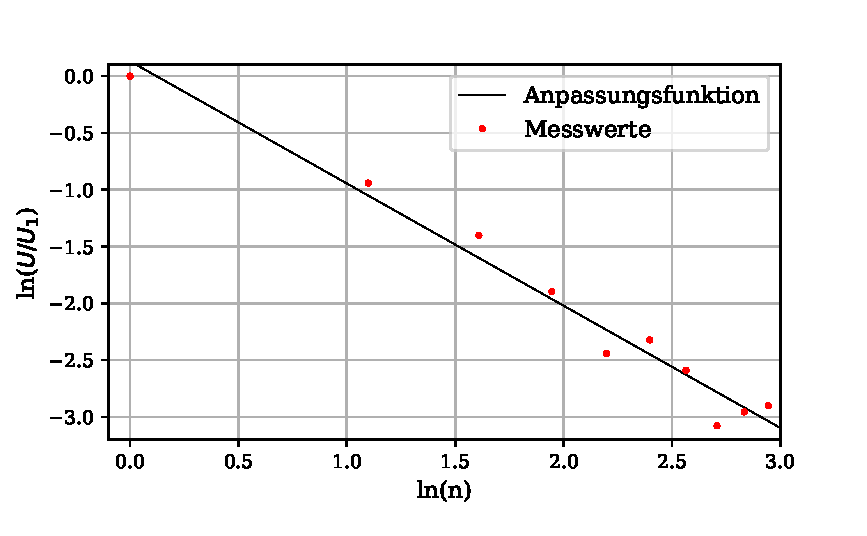
\includegraphics{plot1.pdf}
  \caption{Amplituden der Rechteckspannung doppellogarithmisch aufgetragen gegen die Zahl der Oberwelle.}
  \label{fig:rechteck}
\end{figure}
\noindent Der Ansatz der linearen Regression lautet $y = mx + b$ , und mit Hilfe von Python werden die Parameter und Fehler berechnet, die für die Rechteckschwingung
\begin{align*}
  m &= -1,08 \pm 0,06 \\
  b &= -0,13 \pm 0,14 
\end{align*}
lauten.

\begin{figure}[H]
  \centering
  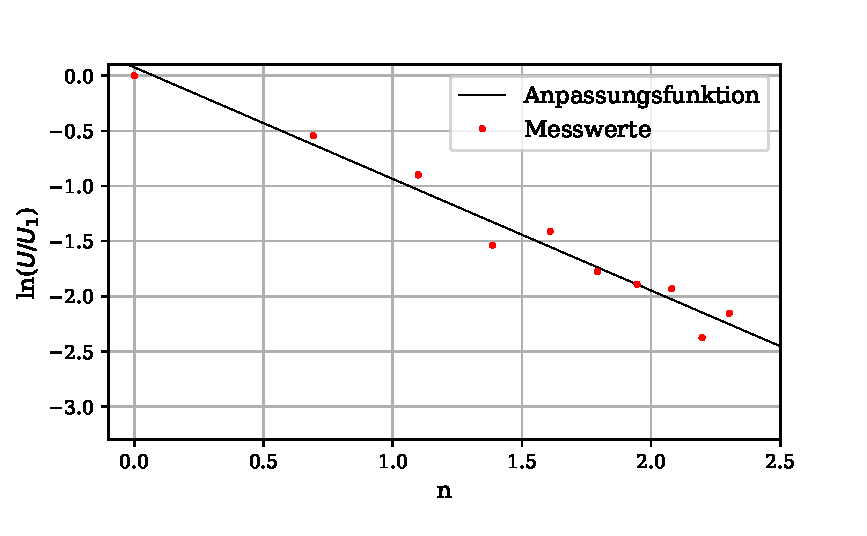
\includegraphics{plot2.pdf}
  \caption{Amplituden der Sägezahnspannung aufgetragen gegen die Zahl der Oberwelle.}
  \label{fig:rechteck}
\end{figure}
Für die Sägezahnspannung ergeben sich die Parameter
\begin{align*}
  m &= -1,01 \pm 0,07 \\
  b &= 0,08 \pm 0,11 .
\end{align*}

\begin{figure}[H]
  \centering
  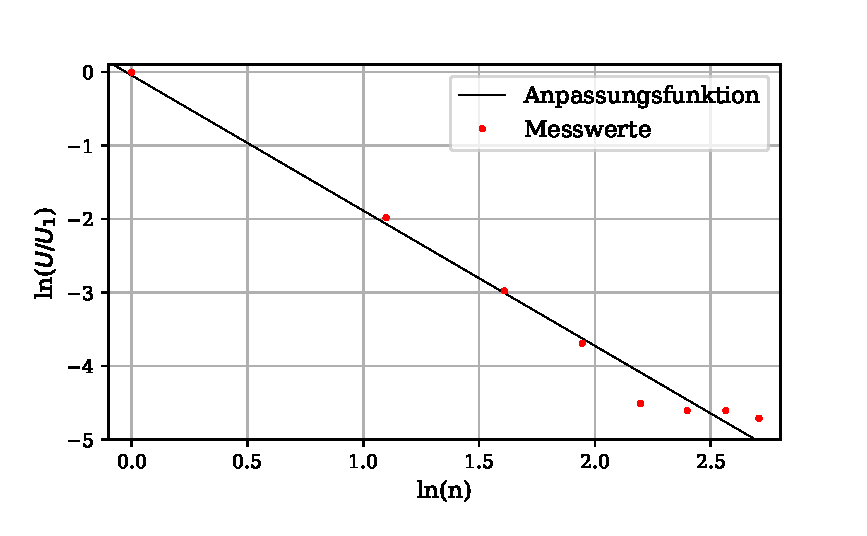
\includegraphics{plot3.pdf}
  \caption{Amplituden der Dreieckspannung aufgetragen gegen die Zahl der Oberwelle.}
  \label{fig:rechteck}
\end{figure}
Zuletzt die Parameter der Dreieckspannung:
\begin{align*}
  m &= -1.84 \pm 0,09 \\
  b &= -0,04 \pm 0,20 .
\end{align*}


\subsection{Fourier-Synthese}
Die Abbildungen 8 bis 10 zeigen die synthetisierten Funktionen. Dabei wird beachtet,
dass die Amplituden der Rechteck- und der Sägezahnspannung mit dem Faktor $\frac{1}{n}$ fallen
und die der Dreieckspannung um den Faktor $\frac{1}{n^2}$. Die Berechnung der notwendigen Spannung erfolgt also durch
Multiplikation der ersten Oberschwingung mit dem jeweiligen Faktor.
Außerdem fallen die Oberschwingungen mit geradem $n$
bei der Rechteck und Dreiecksspannung weg. In Tabelle (2) sind die eingestellten Spannungen aufgelistet.
Bei der Dreieckspannung war es nicht möglich, mehr als 4 Oberwellen einzustellen.
\begin{figure}[H]
  \centering
  \includegraphics[height=5cm]{rechteck.png}
  \caption{Die synthetisierte Rechteckspannung.}
  \label{fig:rechteck}
\end{figure}
\begin{figure}
  \centering
  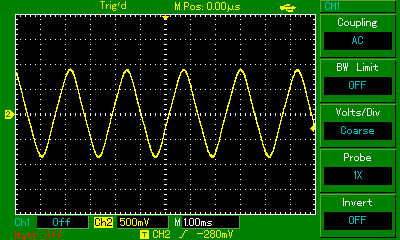
\includegraphics[height=5cm]{Dreieck.png}
  \caption{Die synthetisierte Dreieckspannung.}
  \label{fig:rechteck}
\end{figure}
\begin{figure}
  \centering
  \includegraphics[height=5cm]{Säge.png}
  \caption{Die synthetisierte Sägezahnspannung.}
  \label{fig:rechteck}
\end{figure}



\begin{table}[H]
  \centering
  \caption{Die für die Synthese der Funktionen notwendigen Spannungen.}
  \label{tab:Rechteckspannung}
  \begin{tabular}{c | c | c c}
    \toprule
    Oberwellenzahl $n$ & $U_R/V$ und $U_S/V$ & $U_D/V$   \\
    \midrule
    1 & 0,621 & 0,617\\
    2 & 0,311 & 0,154\\
    3 & 0,207 & 0,069\\
    4 & 0,155 & 0,039\\
    5 & 0,124\\
    6 & 0,104\\
    7 & 0,089\\
    8 & 0,078\\
    9 & 0,069\\
    \bottomrule
  \end{tabular}
\end{table}
